Reflections are one of the distinguishing features of ray tracers, setting them apart from other methods of 3D rendering. When a ray of light hits a perfect reflective surface, like a mirror, the ray is reflected along the surface normal.
\begin{figure}[H]
    \centering
    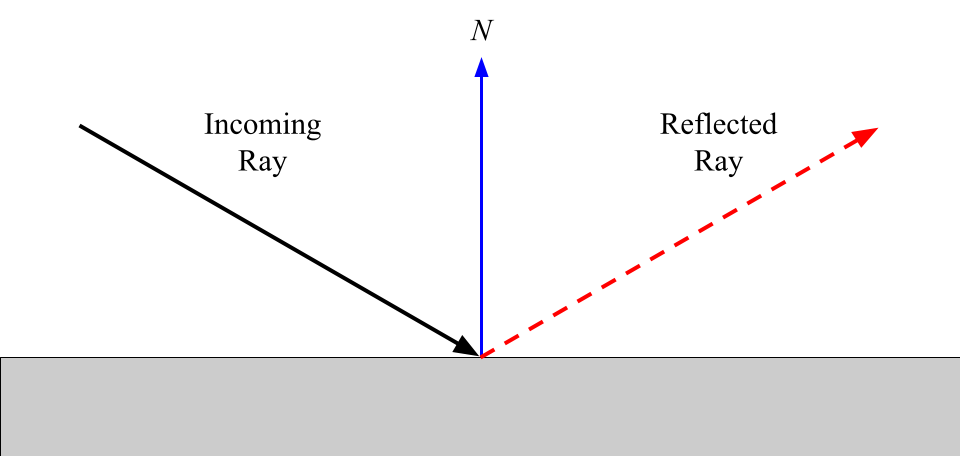
\includegraphics[scale=0.35]{figures/Reflections.png}
    \caption{Result of reflecting a ray over a surface normal}
    \label{fig:reflection_ray}
\end{figure}
\noindent
We can calculate the result of reflecting a ray over a surface normal, $\hat N$ as follows:
$$R = \Vec{P} + t(\hat{D} - 2(\hat{N} \cdot \hat{D})\hat{N})$$
Where $\Vec{P}$ is the intersection point of the incoming ray and the surface and $\hat{D}$ is the direction of the incoming ray. Now, it is important to remember that our rendering approach is the reverse of how light behaves in reality (See 2.2). Given this, we must also approach reflections in the same way. For example, if a camera ray intersects a perfectly reflective sphere, in order to determine the color of the sphere at that point, we must cast the corresponding reflection ray into the scene. There are three different possibilities for how this ray will subsequently behave:
\begin{enumerate}
    \item The reflection ray does not intersect any other object. In this case, the color of the sphere at the intersection point with the camera ray should be the same as the sky color calculated using the reflected ray's $y$ component.
    \item The reflection ray intersects a diffusely shaded, non-reflective object. In this case, the color of the sphere at the intersection point with the camera ray should be the same as the color of the non-reflective object at the intersection point with the reflected ray.
    \item The reflection ray intersects another reflective object. In this case we must recursively cast another reflection ray and compute our final color based on its resulting interactions with the scene.
\end{enumerate}
Note that the third possibility is a recursive case, meaning that when the first reflected ray is cast, we must perform the same calculations on it as the original camera ray. This presents the chance of an infinite recursion depth when reflection rays keep bouncing between adjacent reflective objects, often seen in real life when having two mirrors pointing at each other. This is usually solved by enforcing a maximum amount of light bounces and ignoring reflections beyond the maximum. So far, we have only discussed perfect reflective surfaces. However most objects are not perfectly reflective. We can account for this by defining a shininess coefficient $s$ where $0 \leq s \leq 1$ and $s = 1$ is a perfectly reflective surface while $s = 0$ is a diffuse, non-reflective surface. This allows us to define pixel color as follows by assigning diffuse and reflective shading different weights based on $s$:
$$\text{Color} = (1-s)\Vec{d} + s(\Vec{d}\Vec{r})$$
Where $\Vec{d}$ is a three dimensional color vector representing result of the diffuse lighting calculations discussed earlier and $\Vec{r}$ is a three dimensional color vector representing the color returned from the reflected ray, including subsequent recursive reflections which will employ the same shading equation. Note that the product of $\Vec{d}$ and $\Vec{r}$ is another color vector which is the result of a component-wise multiplication.
\\
\\
\noindent
To demonstrate reflections, we can create a scene with multiple reflective objects to see how they interact. The following image includes 9 spheres with random colors and a shininess coefficient of 0.8, a plane with a checkerboard pattern and a shininess coefficient of 0.3, and a directional light:
\begin{tcolorbox}
\textbf{Note: }Ray-plane intersection was not discussed in the article, however the implementation process is very similar to solving for ray-sphere intersection, just with a different primitive definition.
\end{tcolorbox}
\begin{figure}[H]
    \centering
    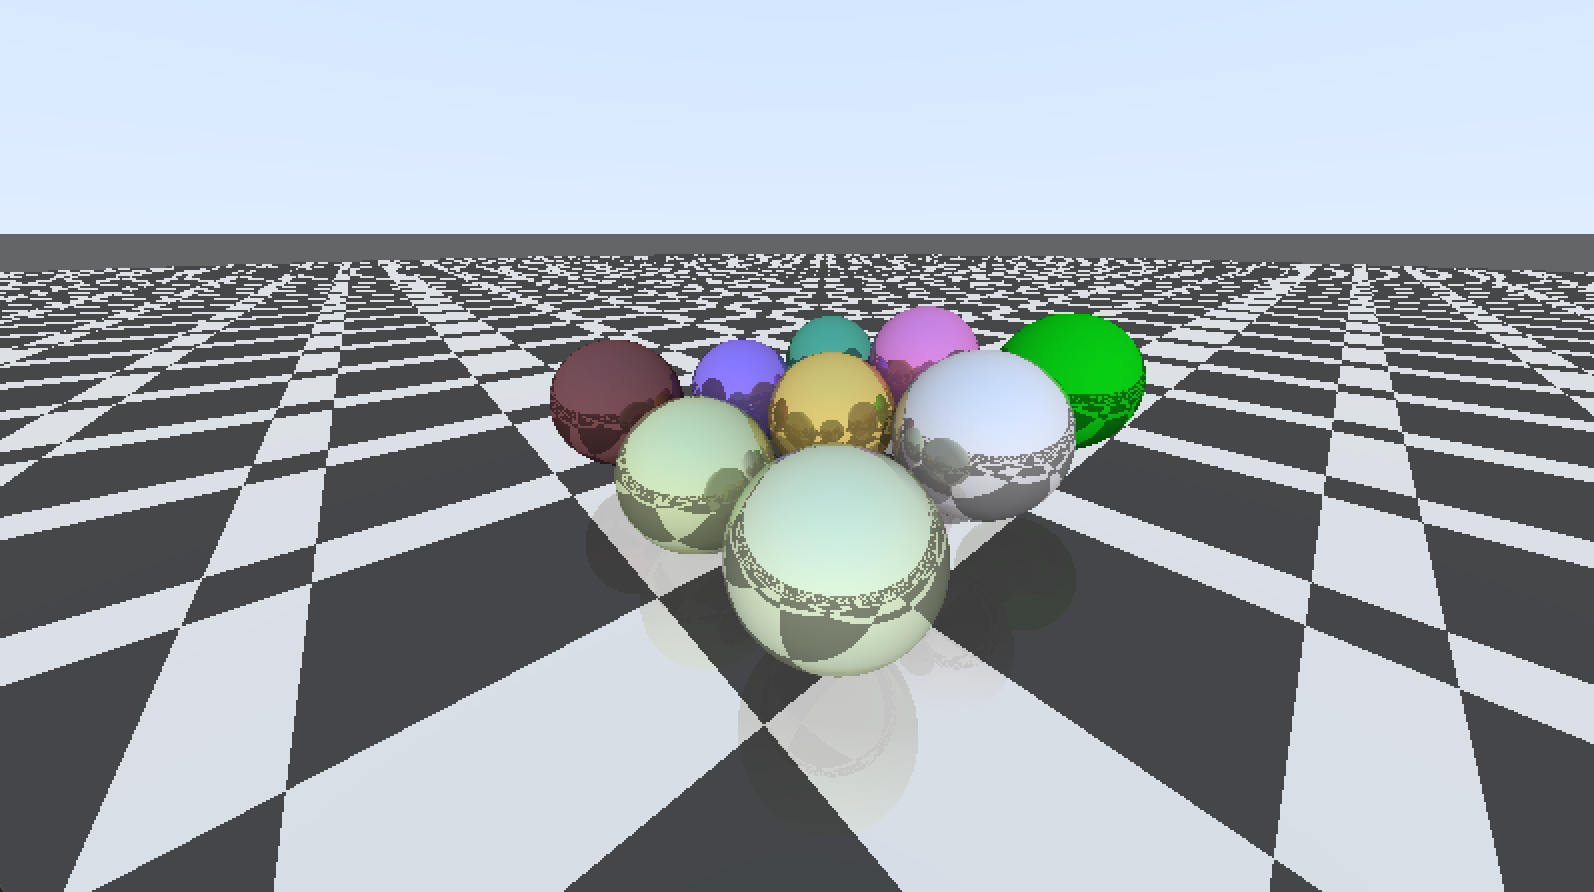
\includegraphics[scale=0.6]{figures/ReflectionDemoScene.png}
    \caption{Demonstration scene highlighting reflections}
    \label{fig:reflect_demo}
\end{figure}
\noindent
If you look closely at the image, particularly the reflections on adjacent spheres, you will notice reflections within the reflections, highlighting the recursive nature of the implementation.